\documentclass[twocolumn,a4paper,dvipdfmx]{ieicejsp}
\usepackage[T1]{fontenc}
\usepackage{lmodern}
\usepackage{textcomp}
\usepackage{latexsym}
\usepackage{float}
\usepackage{graphicx}
\usepackage{amsmath, amssymb}
\usepackage{bm}
\usepackage{upgreek}
\usepackage{caption}
\usepackage{booktabs}
\usepackage{multirow}
\usepackage{tikz}
\usepackage{url}
\usepackage{xcolor}
\usetikzlibrary{positioning, arrows.meta}

\captionsetup{font=small}
\DeclareMathOperator*{\argmax}{arg\,max}
% 修正箇所を赤字で示すコマンド
\newcommand{\add}[1]{{\color{red}#1}}

\title{
    {\bf 物体領域検出とカテゴリアノテーションの分離に基づく，\\WordNetを用いた粒度可変物体アノテーションとCOCO外の物体への拡張}
    {\normalsize \\ Adjustable-Granularity Object Annotation via Decoupled Region Detection and WordNet-Guided Category Annotation, and Its Extension to Objects outside COCO}
}
\author{
    著者名 \\ Author Name
}
\affliate{%
    所属機関名 \\
    Affiliation \\
}

\begin{document}
\maketitle

\begin{abstract}
本稿では，画像中の物体らしい領域を検出するタスクと，その領域のカテゴリをアノテーションするタスクを分離し，WordNetの下位語をたどることで追加学習なしに粒度を変更できる物体アノテーション手法を検討する．
提案手法はクラス非依存の検出にDETRを用い，各領域のクロップのカテゴリをSigLIPのゼロショット分類で推定する．
ハイブリッド手法はYOLOの予測を深さ0とし，YOLOのボックスのクロップに対してSigLIPとWordNetで粒度を変更する．
さらに，YOLOが検出しないCOCO外の物体を，物体らしさに基づく検出器の候補で補う構成を提案する．
COCO 2017 ValidationとLVISのアノテーションを用い，検証用とテスト用に分けた画像で評価した結果，以下を確認した．
第一に，COCOの80クラスの範囲では，ハイブリッド手法がYOLO11xと同じTop-1正解率0.969を保ちつつ，粒度を変更できたインスタンスを提案手法の1.79倍に増やした．
第二に，LVISの細かい粒度の正解に対し，シグモイドの累積確信度で細分化を止めるハイブリッド手法の階層的F値は0.659となり，YOLO11x単体の0.604を上回った．
第三に，COCOで学習したYOLO11xとDETRは閾値を下げてもCOCO外の物体の再現率が2割未満で飽和する一方，OWLv2の物体らしさのスコアは1画像あたり100件で74.3\%に達した．
第四に，YOLO11xのボックスと重ならないOWLv2の候補を加えることで，COCOの物体の精度を保ったまま，COCO外の物体の検出を4.6\%から31.6\%に増やし，粒度の変更の対象にできた．
ただし，検出したCOCO外の物体のうち深さ0を正しく命名できたのは8.1\%であり，命名の語彙と不適切な領域の棄却に課題が残る．
\add{そこで，物体らしさとシグモイドの確信度による候補の棄却と，頻出するカテゴリの語から順に下位語を選ぶ命名，およびSigLIP SO400Mを組み合わせた結果，1画像あたり5件の候補を加える条件で，COCO外の物体の命名を1.7\%から4.1\%に，加えた候補の命名の適合率を3.6\%から8.1\%に向上させた．}
\end{abstract}

\noindent
{\bf キーワード：}物体アノテーション，粒度可変アノテーション，WordNet，SigLIP，YOLO，OWLv2，オープンボキャブラリ

\section{はじめに}
画像データセットに対する物体アノテーションは，画像中のどこに物体が存在するか（物体領域）と，その物体が何であるか（カテゴリ）という，2種類の異なる判断から構成される．
YOLO\cite{ref_YOLO}やDetection Transformer（DETR）\cite{ref_DETR}に代表される一般的な物体検出モデルは，これら2つの判断を単一のモデルに統合し，あらかじめ定めた固定のクラス集合に対して同時に学習する．
そのため，学習時に定めたクラス集合の範囲内では高精度な検出が可能である一方，新たなカテゴリを追加したり，カテゴリの粒度を変更したりする場合には，モデル自体の再学習が必要になる．
例えば，COCO\cite{ref_COCO}の80クラスで学習したYOLOは，ペンギンをbird，ラクダをdogやhorseのように80クラスのいずれかの語でしか表せず，80クラスのいずれにも似ていない物体はそもそも検出しない．

本研究では，物体領域の検出とカテゴリのアノテーションを明確に分離し，検出した領域のクロップに視覚言語モデル（Vision-Language Model，VLM）のゼロショット分類を適用する．
分離により，一度検出した領域に対し，候補語彙を変えるだけでカテゴリのアノテーションを繰り返すことができる．
この性質を用い，WordNet\cite{ref_WordNet}の上位語・下位語の関係をたどることで，追加学習なしに「dog → hunting dog → hound」のように粒度を変更できるアノテーションを実現する．

本稿では，この枠組みを3つの構成で評価する．
第一は，クラス非依存の検出にDETRを用い，深さ0のカテゴリも含めてSigLIP\cite{ref_SigLIP}で推定する提案手法である．
第二は，COCOの範囲で高精度なYOLOの予測を深さ0とし，YOLOのボックスのクロップに対してSigLIPとWordNetで粒度を変更するハイブリッド手法である．
第三は，ハイブリッド手法が検出しないCOCO外の物体を，物体らしさに基づくクラス非依存の検出器で補い，補った領域にも命名と粒度の変更を行う構成である．
比較対象として，YOLO単体を用いる．

本稿の貢献は以下の3点である．
第一に，COCO 2017 Validationと，WordNetのSynsetが付与されたLVIS\cite{ref_LVIS}のアノテーションを用い，YOLO単体，提案手法，ハイブリッド手法の深さ0の精度と，細かい粒度における階層的な精度を，検証用とテスト用に分けた画像で比較する．
第二に，COCO外の物体を見落とさないための検出器として，YOLO，DETR，OWLv2\cite{ref_OWLv2}の物体らしさのスコア，およびGrounding DINO\cite{ref_GroundingDINO}を，1画像あたりのボックス数をそろえて比較し，検出器がCOCO外の物体の粒度変更の上限を決めることを示す．
第三に，YOLOが検出しない領域のみを別の検出器で補う構成により，COCOの物体に対するYOLOの精度を保ったまま，COCO外の物体を検出から粒度の変更まで扱えることを示し，残る課題が命名の語彙にあることを明らかにする．
\add{さらに，加えた候補の棄却と，粗い語から順に選ぶ命名により，COCO外の物体の命名を改善できることを示す．}

本稿の構成は以下のとおりである．
2章で関連研究，3章で提案手法を述べ，4章で実験条件と結果を示す．
5章で考察を行い，6章で本稿をまとめる．

\section{関連研究}
\subsection{閉域的な物体検出モデル}
YOLO\cite{ref_YOLO}は画像を格子に分割し，各格子からボックスとクラスを1回の推論で予測する．
DETR\cite{ref_DETR}はTransformerによる集合予測として検出を定式化し，Non-Maximum Suppression（NMS）を用いずにボックスとクラスを出力する．
いずれも学習時に定めたクラス集合を前提としており，COCO\cite{ref_COCO}で学習したモデルは80クラス以外の語を出力できない．
また，学習データに存在しない物体は背景として扱われるため，検出そのものが行われないことがある．

\subsection{オープンボキャブラリ物体検出とVLM}
Contrastive Language-Image Pre-training（CLIP）\cite{ref_CLIP}は画像とテキストの対の対照学習により，任意の語に対するゼロショット分類を可能にした．
SigLIP\cite{ref_SigLIP}は，候補全体で正規化するソフトマックスの代わりに，画像とテキストの対ごとのシグモイドを用いる目的関数で学習され，語ごとに独立な確信度を与える．
OWL-ViT\cite{ref_OWLViT}やOWLv2\cite{ref_OWLv2}，Grounding DINO\cite{ref_GroundingDINO}は，カテゴリ名をテキストのクエリとして与えることで固定のクラス集合に依存しない検出を行う．
これらのモデルは検出とカテゴリの予測を単一のモデルで同時に行うため，候補語彙や粒度を変えるたびに検出を再実行する必要がある．
一方，OWLv2はテキストに依存しない物体らしさのスコアも出力し，未知の物体を含む領域の候補の生成に用いることができる．
本研究は，検出を1回に限り，候補語彙の変更をクロップの分類のみで行う点で，これらのモデルと異なる．

\section{提案手法}
\subsection{全体設計}
画像$ {\mathbf X} \in {\mathbb R}^{H \times W \times 3} $が与えられたとき，本手法は，物体領域のボックスの集合$ {\mathbb B} = \{ {\mathbf b}_1, \ldots, {\mathbf b}_K \} $を1回の推論で検出し，各ボックス$ {\mathbf b}_k \in {\mathbb R}^4 $について粗い粒度から細かい粒度への単語の列$ ( \hat{v}_k^{(0)}, \hat{v}_k^{(1)}, \ldots ) $を出力する．
ここで，$ H $，$ W $は画像の高さと幅，$ K $は検出数である．
検出とカテゴリのアノテーションを分離するため，候補語彙や粒度を変更しても検出を再実行する必要はない．
本稿で比較する構成の概要を図\ref{fig_pipeline}に示す．

\begin{figure}[t]
    \centering
    \resizebox{\columnwidth}{!}{%
    \begin{tikzpicture}[
            node distance=3mm and 4mm,
            box/.style={draw, rounded corners, align=center, font=\scriptsize, minimum height=6mm, inner sep=2pt},
            arr/.style={-{Stealth[length=1.6mm]}}
        ]
        \node[box] (img) {画像 ${\mathbf X}$};
        \node[box, below=4mm of img] (yolo) {YOLO\\（ハイブリッド）};
        \node[box, left=4mm of yolo] (detr) {DETR\\（提案手法）};
        \node[box, right=4mm of yolo] (owl) {OWLv2\\（補完）};
        \node[box, below=6mm of yolo] (crop) {クロップ ${\mathbf X}_k = \mathrm{Pad}(\mathrm{Crop}({\mathbf X}, {\mathbf b}_k))$};
        \node[box, below=of crop] (root) {深さ0の語 $ \hat{v}_k^{(0)} $：YOLOの語，またはSigLIPで${\mathbb V}_0$から選択};
        \node[box, below=of root] (wn) {$ d = 1, 2, \ldots $ について，SigLIPで\\${\mathbb V}_k^{(d)} = \mathrm{Hyponyms}(\mathrm{synset}(\hat{v}_k^{(d-1)}))$ から選択};
        \node[box, below=of wn] (out) {出力 $ ( \hat{v}_k^{(0)}, \ldots, \hat{v}_k^{(d^\ast)} ) $（累積確信度で停止）};
        \draw[arr] (img) -- (detr);
        \draw[arr] (img) -- (yolo);
        \draw[arr] (img) -- (owl);
        \draw[arr] (detr) -- (crop);
        \draw[arr] (yolo) -- (crop);
        \draw[arr] (owl) -- node[right, font=\tiny, xshift=1mm] {YOLOと重ならない領域} (crop);
        \draw[arr] (crop) -- (root);
        \draw[arr] (root) -- (wn);
        \draw[arr] (wn) -- (out);
    \end{tikzpicture}%
    }
    \caption{本稿で比較する構成の概要．提案手法はDETR，ハイブリッド手法はYOLOのボックスを用い，補完ではYOLOのボックスと重ならないOWLv2の領域を加える．いずれも検出は1回のみ行い，同一のクロップに対してSigLIPによる分類をWordNetの下位語を候補語彙として繰り返す．}
    \label{fig_pipeline}
\end{figure}

\subsection{物体領域の検出}
提案手法では，COCOで学習済みのDETR（ResNet-50）\cite{ref_DETR}を，出力するクラスを用いずにボックスの検出器として用いる．
DETRの各ボックスのスコアは「物体なし」以外のクラスの最大確率であり，閾値$ \theta $を超えるボックスを用いる．
ハイブリッド手法では，COCOで学習済みのYOLO11x\cite{ref_YOLO11}を用い，検出スコア$ s_k $が閾値を超えるボックスと，そのクラス$ y_k $を用いる．
各ボックスのクロップは，VLMの前処理で物体の両端が失われないよう，黒で正方形にパディングした$ {\mathbf X}_k = \mathrm{Pad}(\mathrm{Crop}({\mathbf X}, {\mathbf b}_k)) $とする．
ここで，$ \mathrm{Crop}({\mathbf X}, {\mathbf b}) $は画像$ {\mathbf X} $から$ {\mathbf b} $の範囲を切り出す関数，$ \mathrm{Pad}(\cdot) $は長辺に合わせて黒で埋めて正方形にする関数である．

\subsection{SigLIPによるカテゴリのアノテーション}
カテゴリのアノテーションには，SigLIP\cite{ref_SigLIP}の画像エンコーダ$ g_I $とテキストエンコーダ$ g_T $を用いる．
候補語彙$ {\mathbb V} $の語$ v $を``a photo of a $ \{v\} $''というプロンプト$ t(v) $に埋め込み，クロップ$ {\mathbf X}_k $に対するロジットを

\begin{equation}
    l_v({\mathbf X}_k) = \alpha \cos \bigl( g_I({\mathbf X}_k), g_T(t(v)) \bigr) + \beta
    \label{eq_logit}
\end{equation}

\noindent
とする．
ここで，$ \cos(\cdot, \cdot) $はコサイン類似度，$ \alpha $と$ \beta $は学習済みの温度とバイアスである．
アノテーションする語と確信度を

\begin{equation}
    \hat{v}_k = \argmax_{v \in {\mathbb V}} l_v({\mathbf X}_k), \quad
    p_k = \sigma \bigl( l_{\hat{v}_k}({\mathbf X}_k) \bigr)
    \label{eq_annotation}
\end{equation}

\noindent
とする．
ここで，$ \sigma(x) = 1 / (1 + \exp(-x)) $はシグモイド関数である．
$ p_k $は他の候補語に依存しないため，候補語彙に画像と対応する語が無い場合に小さくなる．
比較として，候補語彙の中で正規化するソフトマックス$ \exp(l_{\hat{v}_k}) / \sum_{u \in {\mathbb V}} \exp(l_u) $を確信度とする場合も評価する．
いずれの場合も$ \hat{v}_k $は同じであり，確信度のみが異なる．

\subsection{WordNetによる粒度の変更}
深さ0の語$ \hat{v}_k^{(0)} $に対応するWordNetのSynsetを$ \mathrm{synset}(\hat{v}_k^{(0)}) $とし，Synset $ s $の直接の下位語の集合を$ \mathrm{Hyponyms}(s) $とする．
深さ$ d \geq 1 $の候補語彙を

\begin{equation}
    {\mathbb V}_k^{(d)} = \mathrm{Hyponyms} \bigl( \mathrm{synset}( \hat{v}_k^{(d-1)} ) \bigr)
    \label{eq_hyponym}
\end{equation}

\noindent
とし，同一のクロップ$ {\mathbf X}_k $に(\ref{eq_annotation})を適用して$ \hat{v}_k^{(d)} $と$ p_k^{(d)} $を得る．
この処理を$ {\mathbb V}_k^{(d)} = \emptyset $となるまで繰り返す．
ただし，深い段階ほど誤りが増えるため，累積確信度

\begin{equation}
    c_k^{(d)} = \prod_{j=0}^{d} p_k^{(j)}
    \label{eq_cumulative}
\end{equation}

\noindent
が閾値$ \tau $以上である最も深い段階$ d^\ast $までを出力し，$ c_k^{(0)} < \tau $の場合はアノテーションを棄却する．
$ \tau $は検証用の画像で選ぶ．
COCOの各カテゴリ名に対応するSynsetは定義文を確認して手動で定め，下位語のSynsetの先頭のレンマ名を候補語とする．

\subsection{比較する3つの構成}
YOLO単体は，YOLOのクラス$ y_k $のみを出力し，粒度を変更しない．
提案手法は，DETRのボックスに対し，COCOの80クラスの集合$ {\mathbb V}^{(0)} $から(\ref{eq_annotation})で深さ0の語を選び，(\ref{eq_hyponym})で粒度を変更する．
ハイブリッド手法は，YOLOのボックスに対し$ \hat{v}_k^{(0)} = y_k $，$ p_k^{(0)} = s_k $とし，(\ref{eq_hyponym})で粒度を変更する．
ハイブリッド手法では，深さ0の精度はYOLOと同じであり，深さ1以降の推定のみをSigLIPとWordNetが担う．

\subsection{COCO外の物体への拡張}
ハイブリッド手法はYOLOが検出したボックスのみを扱うため，YOLOが検出しないCOCO外の物体は粒度の変更の対象にならない．
そこで，クラス非依存の検出器Dの出力$ {\mathbb B}_{\mathrm{D}} $のうち，YOLOのボックス$ {\mathbb B}_{\mathrm{Y}} $のいずれともIoUが0.5未満のボックスを，スコアの上位$ K_{\mathrm{add}} $件まで加える．

\begin{equation}
    {\mathbb B} = {\mathbb B}_{\mathrm{Y}} \cup \mathrm{Top}_{K_{\mathrm{add}}} \Bigl\{ {\mathbf b} \in {\mathbb B}_{\mathrm{D}} \Bigm| \max_{{\mathbf b}' \in {\mathbb B}_{\mathrm{Y}}} \mathrm{IoU}({\mathbf b}, {\mathbf b}') < 0.5 \Bigr\}
    \label{eq_supplement}
\end{equation}

\noindent
YOLOのボックスはハイブリッド手法と同じく扱い，加えたボックスは，深さ0の語をSigLIPで候補語彙$ {\mathbb V}_0 $から選び，(\ref{eq_hyponym})で粒度を変更する．
$ {\mathbb V}_0 $には，再学習を行わずにCOCO外の語を含めるため，WordNetにおいてCOCOのカテゴリと同じ深さにある語を加える．
WordNetの根からの深さは上位語の経路によって異なり，例えばdogは深さ8と13の経路を持つため，木全体で深さを揃えても粒度は揃わない．
そこで，COCOのカテゴリのSynset $ c $ごとに，最長の上位語の経路で2段上の祖先$ a(c) $をとり，$ a(c) $からちょうど2段下にあるSynsetを$ c $と同じ深さの語として

\begin{equation}
    {\mathbb V}_0 = {\mathbb C} \cup \Bigl\{ s \in \bigcup_{c \in {\mathbb C}} {\mathcal H}^{2} \bigl( a(c) \bigr) \Bigm| \phi(s) \Bigr\}
    \label{eq_wordnet_vocab}
\end{equation}

\noindent
とする．
ここで，$ {\mathbb C} $はCOCOの80クラスのSynsetの集合，$ {\mathcal H}^{2}(a) $は$ a $から2段下の下位語の集合である．
$ \phi(s) $は，$ s $が物理的な実体（physical\_entity.n.01）の下位語であり，$ {\mathbb C} $のいずれの上位語・下位語でもなく，SemCor\cite{ref_SemCor}における出現頻度が1以上であることを表す．
例えばdogに対しては，2段上の祖先carnivoreから2段下にあるwolfやfoxが含まれ，birdより深いpenguinや浅いanimalは含まれない．
$ {\mathbb V}_0 $はCOCOの80語を含む681語である．

\begingroup
\color{red}
\subsection{加えた候補の棄却と上から下への命名}
(\ref{eq_supplement})で加えた候補には，GTと対応しない領域や物体の部分が多く含まれる．
そこで，加えた候補$ {\mathbf b}_k $を，OWLv2の物体らしさのスコアが閾値$ o $未満の場合，出力する語のシグモイドの確信度が閾値$ \gamma $未満の場合，および面積の80\%以上が自身より大きい他の出力ボックスに含まれる場合に棄却する．

また，加えた候補には，最初から細かい粒度の語彙$ {\mathbb V}_0 $の中で最も近い語を1つ選ぶのではなく，粗い語から順に選ぶ命名を用いる．
WordNetの最上位の語（thing，object等）はVLMが判別できないため，COCO train2017のキャプションに300回以上出現し，深さが5以上で，下位に語として使えるSynsetを3つ以上持つSynsetと，COCOの80クラスのSynsetからなる274語を出発点の候補$ {\mathbb R} $とする．
ここで，語として使えるSynsetとは，いずれかのレンマがキャプションに5回以上出現し，WordNetにおいて他のSynsetの部分として登録されていないSynsetである．
(\ref{eq_annotation})により$ {\mathbb R} $から深さ0の語を選んだ後，語として使えるSynsetとその上位語のみからなるWordNetの木（8121ノード）で，子の中から(\ref{eq_annotation})により1つずつ選んで葉までたどる．
各段階で選んだ語の兄弟の中でのソフトマックスの確信度が閾値$ \tau_s $未満となった段階で止め，1つ前の段階の語を出力する．
すなわち，語の選択と停止には兄弟の間での比較に適するソフトマックスを，候補の棄却には画像と語の対応の強さを表すシグモイドを用いる．
\endgroup

\section{実験}
\subsection{共通設定}
評価にはCOCO 2017 Validation（5000枚）を用いた．
閾値の選択と結果の報告に同じ画像を用いないよう，seed 42でサンプリングした500枚（以下，dev500）を検証用とし，残りの4500枚を2等分した後半からサンプリングした500枚（以下，test500，GTインスタンス3748件）をテスト用とした．
細かい粒度の評価には，WordNetのSynsetが各カテゴリに付与されたLVIS v1\cite{ref_LVIS}のValidationのアノテーションを用いた．
LVISのアノテーションはCOCO 2017の画像に付与されており，5000枚のうち4809枚に存在する．
dev500と前述の4500枚の前半のうちLVISのアノテーションが存在する2604枚を検証用（以下，lvis\_dev），後半の2148枚をテスト用（以下，lvis\_test）とした．
VLMにはSigLIP-ViT-B/16（WebLIで学習）を，検出器にはDETR（ResNet-50）とYOLO11xを用いた．
DETRの閾値$ \theta $とYOLO11xの閾値は，評価インスタンス数が近くなる組として，$ \theta = 0.5 $とYOLO11xの0.25を主に示す．
GPUにはNVIDIA GeForce RTX 4070 Tiを用い，いずれの手法も追加の学習は行わない．

検出ボックスとCOCOのGTは，IoUが0.5以上の組をハンガリアン法で1対1に対応付けた．
対応したインスタンスについて，深さ0の語がGTのカテゴリと一致する割合をTop-1正解率，深さ0が正解のインスタンス数をGTインスタンスの総数で割った値を正命名率$ r $とした．
また，深さ0が正解であり，かつ下位語を持つため粒度を変更できたインスタンス数を$ N_h $とした．

深さ1以降の評価には，COCOのGTに対応した検出ボックスについて，IoUが0.5以上で，そのSynsetがGTカテゴリのSynsetの真の下位語であるLVISのアノテーションを細かい粒度の正解とした．
例えば，COCOのbirdに対するpigeonである．
インスタンス$ k $について，出力した各段階のSynsetの集合を$ {\mathbb P}_k $，GTカテゴリのSynsetからLVISのSynsetまでの経路上のSynsetの集合を$ {\mathbb G}_k $とし，階層的適合率と階層的再現率\cite{ref_hF}を

\begin{equation}
    hP = \frac{\sum_k |{\mathbb P}_k \cap {\mathbb G}_k|}{\sum_k |{\mathbb P}_k|}, \quad
    hR = \frac{\sum_k |{\mathbb P}_k \cap {\mathbb G}_k|}{\sum_k |{\mathbb G}_k|}
    \label{eq_hierarchical_pr}
\end{equation}

\noindent
とし，その調和平均を$ hF $とした．
LVISのSynsetより細かいSynsetは正誤を判定できないため$ {\mathbb P}_k $から除き，棄却したインスタンスでは$ {\mathbb P}_k = \emptyset $とした．
(\ref{eq_cumulative})の$ \tau $は，lvis\_devで$ hF $が最大となる値を$ 0 $から$ 0.9 $の16通りから選んだ．

\subsection{COCOにおける3つの構成の比較}
表\ref{tab_coco}に，test500における深さ0の結果を示す．

\begin{table}[t]
    \centering
    \caption{test500における深さ0の評価．閾値は提案手法ではDETRの$ \theta $，YOLO11x単体とハイブリッド手法ではYOLO11xの検出スコアの閾値，$ n $は評価インスタンス数，$ N_h $は深さ0が正解で粒度を変更できたインスタンス数である．}
    \label{tab_coco}
    \footnotesize
    \setlength{\tabcolsep}{3pt}
    \begin{tabular}{lccccc}
        \toprule
        手法 & 閾値 & $ n $ & Top-1 & $ r $ & $ N_h $ \\
        \midrule
        YOLO11x単体  & 0.25 & 2572 & 0.969 & 0.665 & 0 \\
        提案手法     & 0.5  & 2736 & 0.527 & 0.385 & 1219 \\
        ハイブリッド & 0.25 & 2572 & 0.969 & 0.665 & 2187 \\
        \midrule
        YOLO11x単体  & 0.7  & 1584 & 0.982 & 0.415 & 0 \\
        提案手法     & 0.97 & 1669 & 0.609 & 0.271 & 867 \\
        ハイブリッド & 0.7  & 1584 & 0.982 & 0.415 & 1360 \\
        \bottomrule
    \end{tabular}
\end{table}

表\ref{tab_coco}から，COCOの80クラスの範囲では，YOLO11xのTop-1正解率0.969に対し，DETRとSigLIPによる提案手法は0.527であった．
提案手法の誤りの多くは，COCOで学習されていないSigLIPのゼロショット分類によるものであり，検出数$ n $は同程度である．
ハイブリッド手法は深さ0の精度をYOLO11xと同じに保ったまま，粒度を変更できたインスタンス$ N_h $を，提案手法の1.79倍（閾値0.25と$ \theta = 0.5 $）および1.57倍（閾値0.7と$ \theta = 0.97 $）に増やした．
YOLO11x単体は深さ0の語のみを出力するため，$ N_h = 0 $である．

\subsection{LVISによる細かい粒度の評価}
表\ref{tab_lvis}と図\ref{fig_lvis_stopping}に，lvis\_testにおける深さ1以降の結果を示す．
評価インスタンス数は，提案手法で489件，YOLO11x単体とハイブリッド手法で481件である．
図\ref{fig_lvis_stopping}の横軸は$ hR $，縦軸は$ hP $であり，曲線は$ \tau $を変化させた停止規則，四角は深さの上限（0〜3）で止める規則，星印はlvis\_devで選んだ$ \tau $である．

\begin{table}[t]
    \centering
    \caption{lvis\_testにおける深さ1以降の評価．深さ1は深さ0が正解のインスタンスにおける深さ1の正解率，到達はLVISのSynsetまで細分化できた割合（停止なし）である．$ hF $の停止なしは下位語の集合が空になるまで出力した場合，$ \tau $はlvis\_devで選んだ$ \tau $による停止規則である．}
    \label{tab_lvis}
    \scriptsize
    \setlength{\tabcolsep}{1.6pt}
    \begin{tabular}{lccccccc}
        \toprule
        & & & & \multicolumn{2}{c}{停止なし} & \multicolumn{2}{c}{$ \tau $による停止} \\
        \cmidrule(lr){5-6} \cmidrule(lr){7-8}
        手法 & 確信度 & 深さ1 & 到達 & $ hP $ & $ hF $ & $ hP $ & $ hF $ \\
        \midrule
        YOLO11x単体  & --         & --    & 0.000 & 0.971 & 0.604 & 0.971 & 0.604 \\
        提案手法     & シグモイド & 0.462 & 0.276 & 0.434 & 0.433 & 0.486 & 0.450 \\
        提案手法     & ソフトマックス & 0.462 & 0.276 & 0.434 & 0.433 & 0.715 & 0.480 \\
        ハイブリッド & シグモイド & 0.405 & 0.389 & 0.602 & 0.619 & 0.757 & 0.659 \\
        ハイブリッド & ソフトマックス & 0.405 & 0.389 & 0.602 & 0.619 & 0.720 & 0.648 \\
        \bottomrule
    \end{tabular}
\end{table}

\begin{figure}[t]
    \centering
    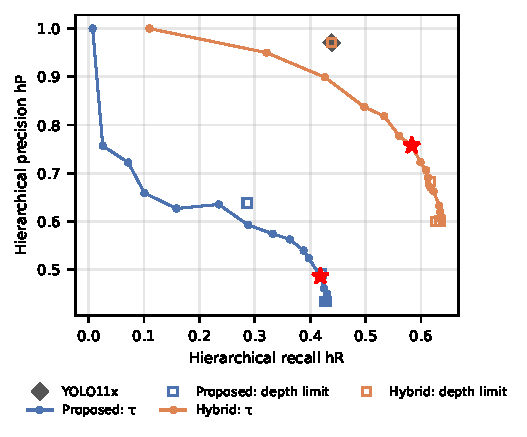
\includegraphics[width=0.9\columnwidth]{figures/fig_lvis_stopping.pdf}
    \caption{lvis\_testにおける階層的再現率$ hR $（横軸）と階層的適合率$ hP $（縦軸）の関係（確信度はシグモイド）．曲線は累積確信度による停止規則，四角は深さの上限（0〜3）による停止規則，星印はlvis\_devで選んだ$ \tau $である．}
    \label{fig_lvis_stopping}
\end{figure}

表\ref{tab_lvis}から，YOLO11x単体は深さ0のみを出力するため$ hP = 0.971 $と高いが，細かい粒度を出力しないため$ hR $は0.438にとどまった．
ハイブリッド手法は，下位語の集合が空になるまで出力すると$ hP $が0.602に下がるが，LVISのSynsetまで細分化できた割合は38.9\%であった．
シグモイドの確信度による停止規則では，$ \tau = 0.05 $で$ hP = 0.757 $，$ hR = 0.583 $となり，$ hF $は0.659とYOLO11x単体の0.604を上回った．
一方，深さ0が正しい場合でも深さ1の推定が正しいのは提案手法で46.2\%，ハイブリッド手法で40.5\%であり，最初の細分化の段階で半数以上を誤った．

確信度の正規化関数の影響を調べるため，深さ0の正誤を最も深い段階の確信度で区別するArea Under the ROC Curve（AUROC）をtest500で求めた．
ハイブリッド手法では，シグモイドで0.617，ソフトマックスで0.480であり，誤った語の下位語のみを候補とする段階でも，シグモイドは画像と語の対応が弱いことを低い確信度として表した．
一方，深さ0が正しい場合の深さ1の正誤を深さ1の確信度で区別するAUROCは，ハイブリッド手法でシグモイドが0.644，ソフトマックスが0.780であり，兄弟の語の間の比較にはソフトマックスが適していた．
提案手法では，シグモイドの深さ0の確信度が小さく，$ \tau $を大きくすると多くのインスタンスが棄却されるため，$ hF $はソフトマックスの0.480に対し0.450であった．

\subsection{COCO外の物体の検出}
YOLO11xやDETRはCOCOで学習されているため，COCO外の物体を背景として扱い，検出しない場合がある．
そこで，lvis\_testの2148枚において，COCOの物体（15842件）と，COCO外の物体（12655件）の検出の再現率を比較した．
COCO外の物体は，LVISのアノテーションのうち，SynsetがCOCOのカテゴリのSynsetの上位語・下位語でなく，レンマ名もCOCOのカテゴリ名と一致しないものである．
比較した検出器は，YOLO11x（閾値0.01），DETR（閾値0.01），OWLv2\cite{ref_OWLv2}（ViT-B/16）のテキストに依存しない物体らしさのスコア，およびテキスト「object.」を与えたGrounding DINO\cite{ref_GroundingDINO}（tiny）である．
いずれもIoU 0.5のクラス非依存のNMSを行い，スコアの上位$ K $件のボックスにIoUが0.5以上のボックスが含まれるGTの割合を再現率とした．

図\ref{fig_recall}に結果を示す．
横軸は1画像あたりのボックス数（対数），縦軸は再現率であり，黒の記号はYOLO11x（閾値0.25）とDETR（$ \theta = 0.5 $）の出力である．

\begin{figure}[t]
    \centering
    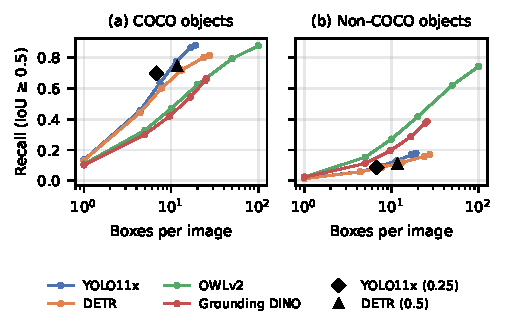
\includegraphics[width=\columnwidth]{figures/fig_recall.pdf}
    \caption{lvis\_testにおける1画像あたりのボックス数（横軸）と再現率（縦軸）の関係．(a)はCOCOの物体，(b)はCOCO外の物体であり，黒の記号はYOLO11x（閾値0.25）とDETR（$ \theta = 0.5 $）の出力である．}
    \label{fig_recall}
\end{figure}

図\ref{fig_recall}(b)から，YOLO11x（閾値0.25）が検出したCOCO外の物体は8.7\%，DETR（$ \theta = 0.5 $）は11.0\%であった．
YOLO11xとDETRは閾値を0.01まで下げても，COCO外の物体の再現率はそれぞれ17.9\%と17.0\%で飽和した．
これに対し，OWLv2の物体らしさのスコアでは，1画像あたり10件で27.1\%，100件で74.3\%であり，Grounding DINO（25.6件で38.5\%）を上回った．
一方，図\ref{fig_recall}(a)から，COCOの物体ではYOLO11xが少ないボックス数で最も高い再現率を示した．
すなわち，COCOの物体にはYOLO11x，COCO外の物体にはOWLv2という役割の分担が有効である．

\subsection{COCO外の物体の命名と粒度の変更}
(\ref{eq_supplement})により，YOLO11x（閾値0.25）のボックスに，各検出器の候補を$ K_{\mathrm{add}} $件加えた構成を評価した．
出力したボックスとGT（COCOの物体とCOCO外の物体）をIoU 0.5以上で1対1に対応付け，COCO外の物体のうち，ボックスと対応した割合（検出），深さ0の語がLVISのSynsetの上位語または自身であった割合（命名），下位語の展開がLVISのSynsetに到達した割合（到達）を求めた．
命名の語彙$ {\mathbb V}_0 $には(\ref{eq_wordnet_vocab})の681語を用い，語彙が既知の場合の参考として，LVISのカテゴリ名（1203語）を語彙とした場合も示す．
提案手法も，DETR（$ \theta = 0.5 $）のボックスを同じ語彙で命名した．
表\ref{tab_open}に$ K_{\mathrm{add}} = 10 $の結果を示す．

\begin{table}[t]
    \vspace{3mm}
    \centering
    \caption{lvis\_testにおけるCOCO外の物体の検出，命名，粒度の変更（$ K_{\mathrm{add}} = 10 $）．COCOはCOCOの物体のうち深さ0が正解の割合，検出・命名・到達はCOCO外の物体12655件に対する割合であり，括弧内はLVISのカテゴリ名を語彙とした場合である．}
    \label{tab_open}
    \scriptsize
    \setlength{\tabcolsep}{1.5pt}
    \begin{tabular}{lcccc}
        \toprule
        構成 & COCO & 検出 & 命名 & 到達 \\
        \midrule
        YOLO11x単体          & 0.649 & 0.046 & 0.000 & 0.000 \\
        ハイブリッド         & 0.649 & 0.046 & 0.000 & 0.000 \\
        提案手法             & 0.231 & 0.070 & 0.006 (0.018) & 0.005 (0.017) \\
        ハイブリッド + YOLO11x & 0.663 & 0.094 & 0.005 (0.011) & 0.005 (0.011) \\
        ハイブリッド + DETR    & 0.660 & 0.087 & 0.004 (0.010) & 0.004 (0.009) \\
        ハイブリッド + OWLv2   & 0.661 & 0.316 & 0.025 (0.084) & 0.023 (0.081) \\
        ハイブリッド + G. DINO & 0.659 & 0.217 & 0.021 (0.057) & 0.019 (0.056) \\
        \bottomrule
    \end{tabular}
\end{table}

表\ref{tab_open}から，YOLO11x単体とハイブリッド手法はCOCO外の物体の4.6\%しか検出せず，検出した物体にもCOCOの語しか与えないため，命名と粒度の変更はいずれも0であった．
OWLv2の候補を加えると，COCO外の物体の検出は31.6\%と6.9倍になり，COCOの物体の正解率も0.649から0.661へわずかに上がった．
すなわち，YOLO11xのボックスと重ならない領域のみを加えることで，COCOの物体に対する精度を損なわずに，検出されなかった物体を粒度の変更の対象にできた．
ただし，検出したCOCO外の物体のうち深さ0を正しく命名できたのは，WordNetの語彙で8.1\%，LVISのカテゴリ名を語彙とした場合でも26.7\%にとどまった．
また，加えたボックスのうちGTと対応したのは21.4\%であり，残りはLVISで注釈されていない物体や物体の部分であった．
$ K_{\mathrm{add}} $を20に増やすと，OWLv2の候補による検出は43.6\%，命名は3.5\%（LVISの語彙で11.1\%）となった．

\begingroup
\color{red}
\subsection{COCO外の物体の命名の改善}
3.7節の棄却と上から下への命名に加え，VLMをSigLIP SO400M（ViT-SO400M-14-SigLIP-384）に変更する構成，クロップのボックスを縦横1.5倍に広げて周辺を含める構成，および深さ1以降のプロンプトに親の語を含める（``a photo of a hound, a type of dog''）構成を評価した．
比較として，(\ref{eq_wordnet_vocab})の語彙から物体の部分を表す語を除き，キャプションに出現する語に限った語彙（COCOの80語を含む435語）を用いる構成も評価した．
YOLO11xのボックスは全構成で共通とし，ハイブリッド手法と同じくシグモイドの累積確信度で$ \tau = 0.05 $まで出力した．

評価には，COCOの物体とCOCO外の物体を合わせた全てのGTと，棄却されなかった全ての出力ボックスを用いた．
出力ボックスとGTをIoU 0.5以上で1対1に対応付け，出力した語とGTのSynsetのそれぞれについて，自身と全ての上位語のうち深さ4以上のSynsetの集合から(\ref{eq_hierarchical_pr})と同様に$ hP $と$ hR $を求めた．
GTと対応しない出力ボックスは$ hP $の分母のみに，対応する出力の無いGTは$ hR $の分母のみに含めた．
したがって，粗い語であっても正しい上位語を出力すれば部分的に正解となり，誤った細かい語は不正解となる．
ただし，LVISの注釈は網羅的でないため，全体の$ hF $が最大となる閾値を選ぶと，加えた候補がほぼ全て棄却される．
そこで，1画像あたりに加える候補の数の上限（予算）$ B $を定め，lvis\_devの1000枚で，予算以下となる閾値の組のうちCOCO外の物体の$ hR $が最大となる組を選び，lvis\_testで評価した．
探索した閾値は，$ K_{\mathrm{add}} \in \{1, 2, 5, 10, 20\} $，$ o \in \{0, 0.1, 0.2, 0.3\} $，$ \gamma \in \{0, 0.003, 0.01, 0.03, 0.1\} $，包含による棄却の有無，$ \tau_s \in \{0, 0.5, 0.7, 0.9\} $および深さ0のみを出力する設定である．

\begin{table}[t]
    \centering
    \caption{lvis\_testにおけるCOCO外の物体の命名の改善．追加は1画像あたりに加えた候補の数，命名はCOCO外の物体12655件のうち深さ0が正しい上位語となった割合，$ hR $はCOCO外の物体の階層的再現率，適合率は加えた候補のうちGTと対応し正しい上位語を出力した割合である．}
    \label{tab_naming}
    \scriptsize
    \setlength{\tabcolsep}{1.4pt}
    \resizebox{\columnwidth}{!}{%
    \begin{tabular}{lcccccccc}
        \toprule
        & \multicolumn{4}{c}{$ B = 2 $} & \multicolumn{4}{c}{$ B = 5 $} \\
        \cmidrule(lr){2-5} \cmidrule(lr){6-9}
        構成 & 追加 & 命名 & $ hR $ & 適合率 & 追加 & 命名 & $ hR $ & 適合率 \\
        \midrule
        上位$ K $件（表\ref{tab_open}）& 2.00 & 0.010 & 0.047 & 0.054 & 5.00 & 0.017 & 0.073 & 0.036 \\
        + 棄却                          & 1.90 & 0.014 & 0.056 & 0.081 & 4.57 & 0.023 & 0.084 & 0.052 \\
        + 上から下への命名               & 1.88 & 0.014 & 0.053 & 0.080 & 4.92 & 0.031 & 0.081 & 0.065 \\
        + SO400M                         & 1.88 & 0.016 & 0.054 & 0.092 & 4.95 & 0.041 & 0.085 & 0.081 \\
        + SO400M，拡大，親の語           & 1.99 & 0.019 & 0.056 & 0.114 & 4.85 & 0.035 & 0.086 & 0.081 \\
        \midrule
        語彙の限定 + SO400M（参考）      & 1.93 & 0.011 & 0.050 & 0.083 & 4.83 & 0.021 & 0.076 & 0.054 \\
        \bottomrule
    \end{tabular}%
    }
\end{table}

\begin{figure}[t]
    \centering
    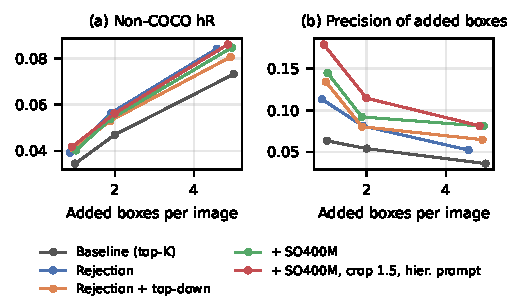
\includegraphics[width=\columnwidth]{figures/fig_budget.pdf}
    \caption{lvis\_testにおける1画像あたりに加えた候補の数（横軸）と，(a) COCO外の物体の階層的再現率，(b) 加えた候補のうちGTと対応し正しい上位語を出力した割合（縦軸）の関係．各点は予算$ B = 1, 2, 5 $でlvis\_devにより選んだ閾値の結果である．}
    \label{fig_budget}
\end{figure}

表\ref{tab_naming}と図\ref{fig_budget}に結果を示す．
棄却を行うと，$ B = 2 $においてCOCO外の物体の$ hR $は0.047から0.056へ，加えた候補の適合率は5.4\%から8.1\%へ向上した．
選ばれた閾値はいずれも$ o \geq 0.2 $であり，OWLv2の物体らしさのスコアによる棄却が有効であった．
一方，包含による棄却はいずれの予算でも選ばれなかった．
上から下への命名は，$ B = 5 $において命名を2.3\%から3.1\%へ，適合率を5.2\%から6.5\%へ高めた．
さらにVLMをSO400Mに変えると，命名は4.1\%，適合率は8.1\%となり，上位$ K $件をそのまま加える場合のそれぞれ2.4倍と2.2倍であった．
一方，同じSO400Mでも，限定した語彙から最初に1語を選ぶ命名では命名が2.1\%にとどまった．
すなわち，VLMの能力を上げた場合に，粗い語から順に選ぶ命名の効果が大きくなった．
クロップの拡大と親の語を含むプロンプトを組み合わせると，$ B = 1 $と$ B = 2 $の適合率は17.9\%と11.4\%で最も高くなった．
いずれの構成でもCOCOの物体の$ hR $は加える前の0.654から0.66〜0.69へわずかに向上し，COCOの物体に対する精度は損なわれなかった．
ただし，改善後もCOCO外の物体の命名は4.1\%であり，検出した物体の多くは依然として正しく命名できていない．
\endgroup

\subsection{定性的結果}
図\ref{fig_qualitative}に，COCO外の物体を主な被写体とする実画像（Wikimedia Commons）に対する，YOLO11xにOWLv2の候補を加えた構成の結果を示す．
青はYOLO11xのボックス，赤は加えた候補のうち物体らしさのスコアの上位3件である．
YOLO11xはラクダをdog，カンガルーをbearとsheepとし，2枚の灯台の画像では何も検出しなかった．
OWLv2の候補により灯台の領域が検出され，1枚目ではtower → beacon（WordNetでlighthouseと同じSynset）まで細分化された．
一方，2枚目の灯台はlight → anchor lightとなり，建物の屋根や地面にはcoatingやditchのような物体の名前として不適切な語が与えられた．
ラクダとカンガルーは，同じ深さの語彙に含まれないためYOLO11xの語のままであり，加えた候補も手綱や子どもの個体，地面に対応した．

\begin{figure*}[t]
    \centering
    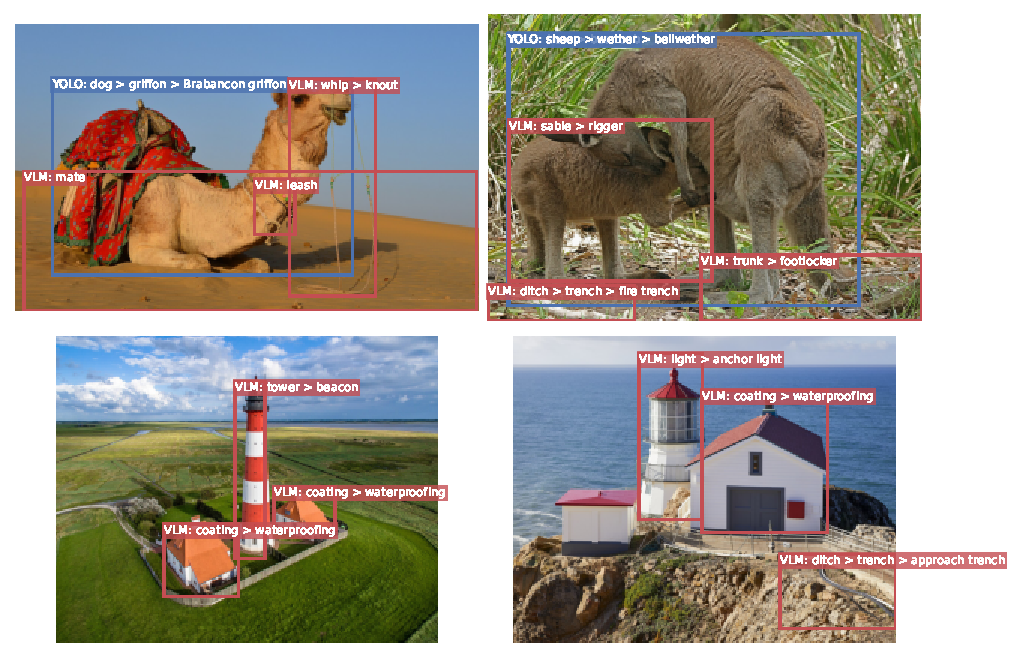
\includegraphics[width=0.85\linewidth]{figures/fig_qualitative.pdf}
    \caption{COCO外の物体を主な被写体とする実画像に対する，YOLO11xにOWLv2の候補を加えた構成の結果．青はYOLO11x（閾値0.25）のボックスとハイブリッド手法による粒度の変更，赤は加えた候補のうち物体らしさのスコアの上位3件とSigLIPによる命名と粒度の変更である．画像はWikimedia Commons（CC BY-SA 3.0/4.0）より取得した．}
    \label{fig_qualitative}
\end{figure*}

\section{考察}
\subsection{3つの構成の使い分け}
COCOの80クラスの範囲では，深さ0の精度はYOLO11xが提案手法を大きく上回り，その差は検出器ではなくカテゴリの分類器に起因する．
ハイブリッド手法は，深さ0をYOLO11xに任せることでこの差を解消し，粒度を変更できたインスタンスを提案手法の1.57〜1.79倍に増やした．
したがって，深さ0のカテゴリが閉域の検出器の語彙に含まれる場合はハイブリッド手法が適する．
一方，提案手法はDETRのボックスに対して任意の語彙から深さ0を選べるため，深さ0の語彙自体をCOCOから変更したい場合に用いることができる．
ただし，DETRもCOCOで学習されているため，提案手法でもCOCO外の物体の検出は11.0\%にとどまり，語彙を自由にできることがCOCO外の物体への対応に直結しなかった．

\subsection{COCO外の物体への対応}
COCO外の物体の粒度の変更は，検出，深さ0の命名，下位語の選択の3段階の積で決まる．
検出の段階では，COCOで学習した検出器の閾値を下げても再現率は2割未満で飽和し，見落とした物体は後段で回復できない．
物体らしさを学習したOWLv2の候補をYOLO11xのボックスと重ならない領域に限って加えることで，COCOの物体の精度を保ったまま検出を6.9倍にでき，検出器が粒度の変更の上限を決めることが確認された．
一方，命名の段階では，検出したCOCO外の物体のうち深さ0を正しく命名できたのは8.1\%であった．
LVISのカテゴリ名を語彙とした場合でも26.7\%であるため，命名の誤りは語彙の不足だけでなく，SigLIP-ViT-B/16による小さな領域の分類の難しさにも起因する．
WordNetの同じ深さの語彙には，物体の部分（leg，screen）や多義の語（coating，slit）が含まれ，加えた候補の約8割はGTと対応しない領域であったため，これらの領域に不適切な語が与えられた．
したがって，物体の名前としての用いられやすさを考慮した語彙の選択と，確信度による領域の棄却が必要である．
\add{4.6節の結果から，物体らしさのスコアによる棄却は加えた候補の適合率を高め，粗い語から順に選ぶ命名は，VLMの能力が高い場合に，最初から細かい語を1つ選ぶ命名を大きく上回った．一方，キャプションに出現する語への語彙の限定は，最初から1語を選ぶ命名では効果が無く，語彙の大きさよりも，選ぶ順序と停止の仕組みが重要であった．ただし，改善後もCOCO外の物体の命名は4.1\%にとどまり，検出した物体の多くは正しく命名できていない．}

\subsection{今後の課題}
第一に，深さ0の語彙を，画像データセットにおける出現頻度や語の具体性に基づいて選び直すことが挙げられる．
第二に，\add{4.6節で評価した棄却は，加える候補の数の予算に対してCOCO外の物体の再現率を最大化する閾値を選んだものであり，LVISの注釈が網羅的でないため加えた候補の適合率を正確に評価できていない．網羅的な注釈を持つデータセットでの評価と，}加えた候補のうち物体でない領域や物体の部分を，シグモイドの確信度やOWLv2の物体らしさのスコアにより棄却する規則の設計が挙げられる．
第三に，シグモイドは誤った枝の検出に，ソフトマックスは兄弟の語の間の比較に適するため，両者を組み合わせた停止規則が挙げられる．
第四に，より規模の大きいVLMや，LVIS以外の細かい粒度のアノテーションを持つデータセットでの評価が挙げられる．

\section{おわりに}
本稿では，物体領域の検出とカテゴリのアノテーションを分離し，WordNetの下位語をたどることで追加学習なしに粒度を変更できる物体アノテーションを，DETRとSigLIPによる提案手法，YOLOの予測を深さ0とするハイブリッド手法，およびYOLO単体で比較した．
COCO 2017 Validationでは，ハイブリッド手法が深さ0のTop-1正解率0.969をYOLO11xと同じく保ちつつ，粒度を変更できたインスタンスを提案手法の1.79倍に増やした．
LVISの細かい粒度の正解による評価では，シグモイドの累積確信度による停止規則を用いたハイブリッド手法の階層的F値が0.659となり，YOLO11x単体の0.604を上回った．
COCO外の物体については，COCOで学習したYOLO11xとDETRは閾値を下げても再現率が2割未満で飽和する一方，OWLv2の物体らしさのスコアによる候補をYOLO11xのボックスと重ならない領域に限って加えることで，COCOの物体の精度を保ったまま，COCO外の物体の検出を4.6\%から31.6\%に増やし，粒度の変更の対象にできることを示した．
一方，検出したCOCO外の物体のうち深さ0を正しく命名できたのは8.1\%であり，語彙の選択と不適切な領域の棄却が今後の課題である．
\add{これに対し，物体らしさとシグモイドの確信度による候補の棄却，頻出するカテゴリの語から順に下位語を選ぶ命名，およびSigLIP SO400Mを組み合わせることで，1画像あたり5件の候補を加える条件で，COCO外の物体の命名を1.7\%から4.1\%に，加えた候補の命名の適合率を3.6\%から8.1\%に向上させた．}

\vspace{-1mm}
\begin{thebibliography}{99}

    \bibitem{ref_YOLO}
    J. Redmon, S. Divvala, R. Girshick, and A. Farhadi,
    ``You Only Look Once: Unified, Real-Time Object Detection,''
    in {\it Proc. IEEE Conference on Computer Vision and Pattern Recognition (CVPR)}, 2016.

    \bibitem{ref_DETR}
    N. Carion, F. Massa, G. Synnaeve, N. Usunier, A. Kirillov, and S. Zagoruyko,
    ``End-to-End Object Detection with Transformers,''
    in {\it Proc. European Conference on Computer Vision (ECCV)}, 2020.

    \bibitem{ref_COCO}
    T.-Y. Lin, M. Maire, S. Belongie, J. Hays, P. Perona, D. Ramanan, P. Doll\'{a}r, and C. L. Zitnick,
    ``Microsoft COCO: Common Objects in Context,''
    in {\it Proc. European Conference on Computer Vision (ECCV)}, 2014.

    \bibitem{ref_WordNet}
    G. A. Miller,
    ``WordNet: A Lexical Database for English,''
    {\it Communications of the ACM}, vol. 38, no. 11, pp. 39--41, 1995.

    \bibitem{ref_SigLIP}
    X. Zhai, B. Mustafa, A. Kolesnikov, and L. Beyer,
    ``Sigmoid Loss for Language Image Pre-Training,''
    in {\it Proc. IEEE/CVF International Conference on Computer Vision (ICCV)}, pp. 11975--11986, 2023.

    \bibitem{ref_LVIS}
    A. Gupta, P. Doll\'{a}r, and R. Girshick,
    ``LVIS: A Dataset for Large Vocabulary Instance Segmentation,''
    in {\it Proc. IEEE/CVF Conference on Computer Vision and Pattern Recognition (CVPR)}, pp. 5356--5364, 2019.

    \bibitem{ref_OWLv2}
    M. Minderer, A. Gritsenko, and N. Houlsby,
    ``Scaling Open-Vocabulary Object Detection,''
    in {\it Proc. Advances in Neural Information Processing Systems (NeurIPS)}, 2023.

    \bibitem{ref_GroundingDINO}
    S. Liu, Z. Zeng, T. Ren, F. Li, H. Zhang, J. Yang, C. Li, J. Yang, H. Su, J. Zhu, and L. Zhang,
    ``Grounding DINO: Marrying DINO with Grounded Pre-Training for Open-Set Object Detection,''
    in {\it Proc. European Conference on Computer Vision (ECCV)}, 2024.

    \bibitem{ref_CLIP}
    A. Radford, J. W. Kim, C. Hallacy, A. Ramesh, G. Goh, S. Agarwal, G. Sastry, A. Askell, P. Mishkin, J. Clark, G. Krueger, and I. Sutskever,
    ``Learning Transferable Visual Models From Natural Language Supervision,''
    in {\it Proc. International Conference on Machine Learning (ICML)}, 2021.

    \bibitem{ref_OWLViT}
    M. Minderer, A. Gritsenko, A. Stone, M. Neumann, D. Weissenborn, A. Dosovitskiy, A. Mahendran, A. Arnab, M. Dehghani, Z. Shen, X. Wang, X. Zhai, T. Kipf, and N. Houlsby,
    ``Simple Open-Vocabulary Object Detection with Vision Transformers,''
    in {\it Proc. European Conference on Computer Vision (ECCV)}, 2022.

    \bibitem{ref_YOLO11}
    G. Jocher, J. Qiu, and A. Chaurasia,
    ``Ultralytics YOLO,''
    2023, \url{https://github.com/ultralytics/ultralytics}.

    \bibitem{ref_SemCor}
    G. A. Miller, C. Leacock, R. Tengi, and R. T. Bunker,
    ``A Semantic Concordance,''
    in {\it Proc. ARPA Workshop on Human Language Technology}, pp. 303--308, 1993.

    \bibitem{ref_hF}
    S. Kiritchenko, S. Matwin, R. Nock, and A. F. Famili,
    ``Learning and Evaluation in the Presence of Class Hierarchies: Application to Text Categorization,''
    in {\it Proc. Canadian Conference on Artificial Intelligence}, pp. 395--406, 2006.

\end{thebibliography}


\end{document}
